\chapter{Regulatory Test System}  \label{chap:3}

The standard Regulatory Test System (TS8997) by \acs{RS}\textregistered{} verifies technologies typically used in wideband wireless devices, i.e. devices with a radio interface, in the 2.4 GHz and 5 GHz band: \acs{WLAN} \acs{IEEE} 802.11a/b/g/n/ac, Bluetooth\textregistered, wireless video transmission and radio remote control. The test system consists of a Signal Generator, Spectrum Analyzer,  \acf{CMW}, and a Switching Unit (OSP-B157W8). My thesis investigates the approach of normalized measurements using the \acs{RF} Shielded Box and a Switching Unit (OSP-B157WN), which is an extension to the current standard regulatory test system. This extension is required for the normalized measurements.

\begin{figure}[H]
\centering
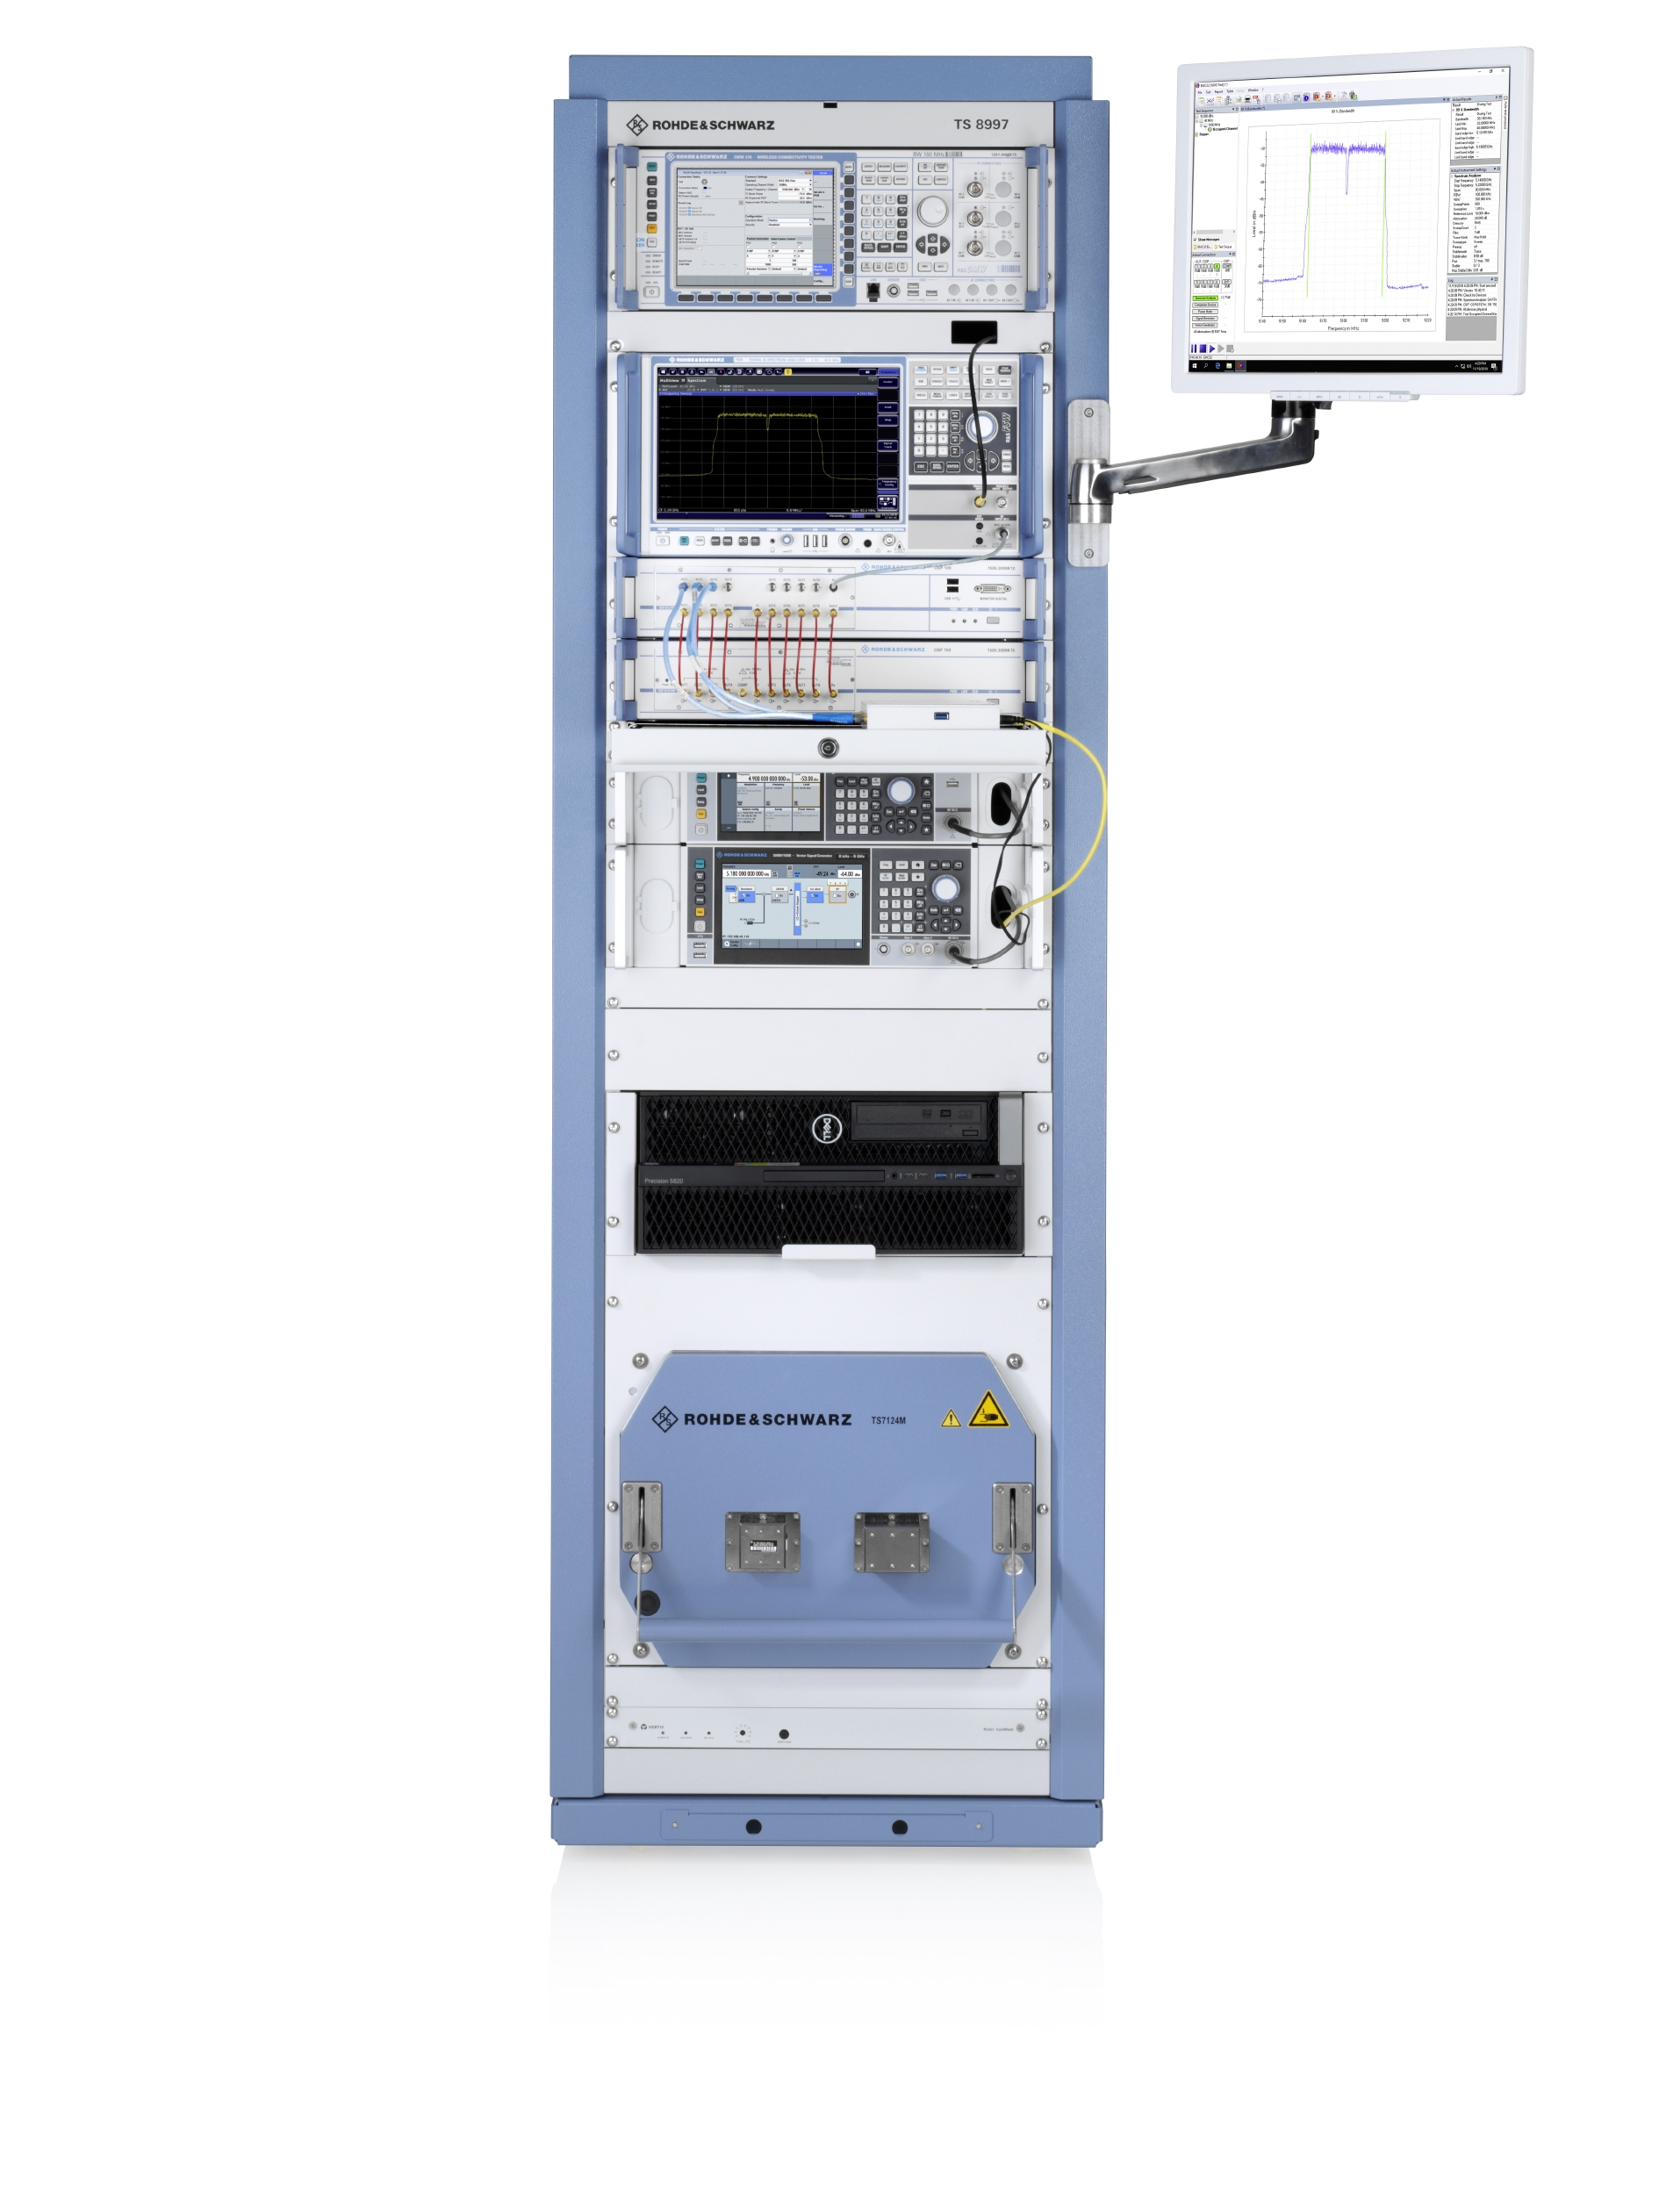
\includegraphics[width=0.5\textwidth]{TestSystem.jpg}
\caption{\acs{RS}\textregistered{} Test System - TS8997}
\label{fig:testsystem}
\end{figure}

This chapter includes all the instruments / equipments required for this thesis. Each section describes in brief about the instrument / software.

\section{WMS32 Software Suite}
\label{sec:wms32}
WMS32 software suite comes with the standard regulatory test system (TS8997). The software features loading, starting, and stopping, pausing, and saving of tests. This software is used only for conducted measurements. In this thesis, this software is not made use of because the software is optimized for end users and one cannot have full control over the settings of the instrument which is very much required for academic research. It is not possible to debug and check results at different stages during the tests if the WMS32 software is used. The only way it would be possible is by learning the source code of the software and trying to debug it via the source code. But, since it is not very convenient to do that, I wrote my code from scratch for all the measurement tests. The figure below shows the \acs{GUI} of the WMS32 software.

\begin{figure}[H]
\centering
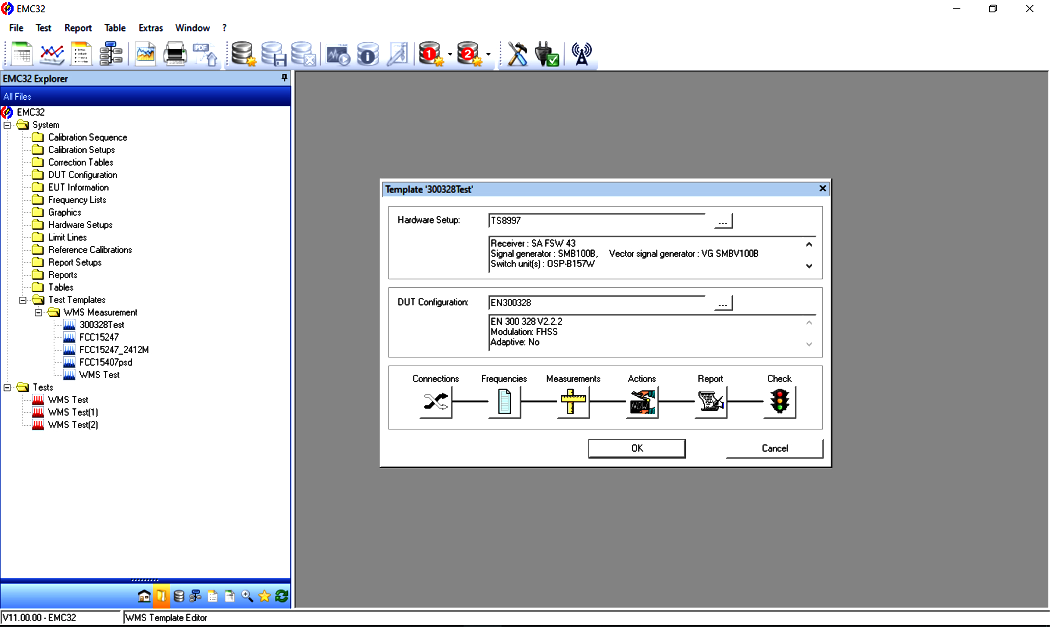
\includegraphics[width=0.8\textwidth]{wms32.pdf}
\caption{\acs{RS} software suite - WMS32}
\label{fig:softwaresuite}
\end{figure}

\section{Spectrum Analyzer}
The analyzer measures the signal either in the frequency domain or in the time domain (zero span). A MATLAB\textregistered{} script is written to remotely access the instrument. The MATLAB\textregistered{} code then calculates the power and bandwidth. The \acf{SCPI} commands for each task (i.e. changing the frequency, span, etc.) are provided in the manual. Few important functions used in this thesis are explained below.

\subsection{Trace Mode}
Signals that are varying are dealt with by setting the trace mode in the spectrum analyzer. The available modes are Clear/Write, \acs{Max-Hold}, or Average.
\begin{enumerate}
  \item Clear/Write is used when new overwritten values are needed on every sweep. It shows what is coming in, as it happens. The change in the signal during the sweep causes the trace level to change. 
  \item \acs{Max-Hold} stores the sweep only when the new value is greater than the previous one. The maximum value of the signal can be thus determined over several sweeps. This makes the trace continue to increase as various signals come and go. If a signal shows up once, it is saved on the Max-Hold trace. Setting trace 1 to normal, and trace 2 to \acs{Max-Hold} is useful in many situations, as it shows both the current power level and the excursion limits.  
  \item Average Mode activates the averaging function of the trace. The average is formed over several sweeps. The number of sweeps is selected by the user. The average model is good, but a slow, tool to remove random noise and highlight constant signals. It is great when the signal you are interested in is near the noise floor of the instrument.  
  \end{enumerate}

\subsection{Detector Settings}
Spectrum analyzers normally sample many more data points than they can display on the screen - tens, hundreds, or thousands of times more. This implies that the displayed trace needs to be summarized in some manner to choose the value to be displayed on each pixel of the screen. This is done by the detectors. The six main detectors settings are:
\begin{enumerate}
  \item Max Peak / Min Peak: They determine the largest of all positive (max peak) or the smallest of all negative (min peak) peak values of the levels measured at the individual frequencies which are displayed on one sample point (or within a pixel). Even if wide spans are displayed with very narrow resolution bandwidth (span/\acs{RBW} >> number of pixels on the frequency axis), no input signals are lost. Therefore this type of detector is particularly useful for \acs{EMC} measurements. This detection method is a good complement to a acs{Max-Hold} trace.
  \item Auto Peak: This detector combines the peak detectors. The maximum peak detector and the minimum peak detector simultaneously determine the maximum and the minimum level within a displayed test point and display it as a single measured value. 
  \item Sample: The detector routes through the sampled data without any further evaluation and either displays them directly or, for reasons of speed in case of short sweep times, first writes them into memory and processes them subsequently. If the span to be displayed is much greater than the resolution bandwidth (span/\acs{RBW} >> number of pixels on the frequency axis), input signals are no longer reliably detected. The same unreliability applies when too large tuning steps of the local oscillator are chosen. In this case, signals may not be displayed at the correct level or may be completely lost. This is required by some standards but is not so useful for spectrum monitoring. 
  \item \ac{RMS}: This detector forms the acs{RMS} value of the measured values within a pixel. To do so, the instrument uses the linear voltage after envelope detection. The sampled linear values are squared, summed and the sum is divided by the number of samples (= \acs{RMS}). For logarithmic display, the logarithm is formed from the square sum. For linear display, the root mean square value is displayed. Each sweep point thus corresponds to the power of the measured values summed up in the sweep point. 
  \item Average: The average detector calculates the linear average of all samples contained in a sweep point. To this effect, the instrument uses the linear voltage after envelope detection. The sampled linear values are summed up and the sum is divided by the number of samples (= linear average value). For logarithmic display, the logarithm is formed from the average value. For linear display, the average value is displayed. Each sweep point thus corresponds to the average of the measured values summed up in the sweep point. The average detector supplies the average value of the signal irrespective of the waveform (\acs{CW} carrier, modulated carrier, white noise, or impulsive signal). 
  \end{enumerate}
  
\begin{figure}[H]
\centering
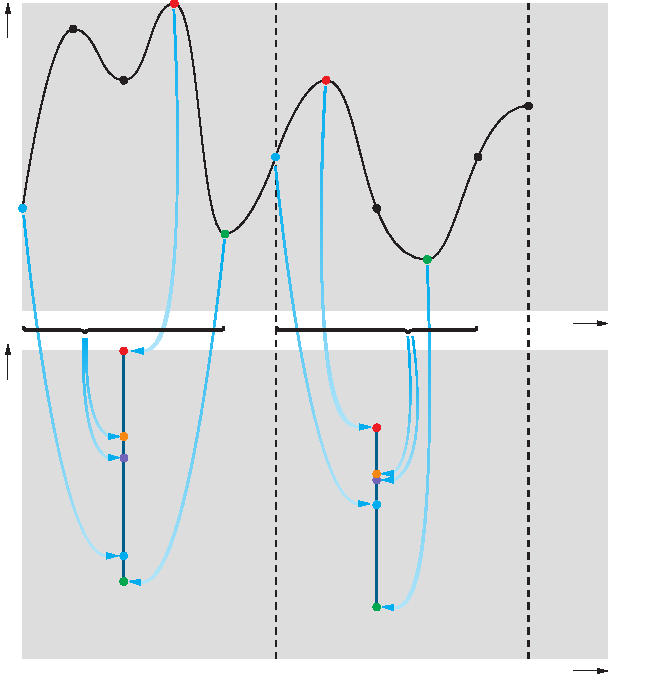
\includegraphics[width=0.7\textwidth]{detectorSetting.pdf}
\caption{Selection of sample to be displayed as a function of detector used}
\label{fig:detectorSettings}
\end{figure}

The choice of detector setting depends on the expected signal. If the signal has a stochastic signal (noise), then the \acs{RMS}-detector is always the best option. This is because the \acs{RMS} detector allows measurement of the actual power of an input signal irrespective of its temporal characteristic. If the crest factor is unknown, the power of random signals (whose instantaneous values are not in line with the Gaussian distribution) can only be determined using an \acs{RMS} detector. When using a sample or max peak detector, the relationship between \acs{RMS} value and peak value must be precisely known for determining the power of signals with random instantaneous value. This knowledge is not required when using an \acs{RMS} detector. The \acs{RMS} value displayed by a specific pixel is calculated from all samples pertaining to this pixel. By increasing the sweep time, the number of samples available for the calculation is increased, thus allowing smoothing of the displayed trace. Smoothing by reducing the video bandwidth or by averaging over several traces is neither permissible nor necessary with the \acs{RMS} detector. The measurement results would be falsified since the displayed values would be too low (max. 2.51 dB). To avoid any falsification of results, the video bandwidth should be at least three times the resolution bandwidth when using the \acs{RMS} detector. If the signal is harmonic, the Max Peak-detector is the correct choice. 


\section{Signal Generator}
\acs{RS}\textregistered{} SMB100A acts as a blocker instrument in this research topic. It is, like other instruments also remotely accessed using \acs{SCPI} commands via a MATLAB\textregistered{} script. It operates in the frequency range of 100 kHz to 40 GHz. The maximum output power is +27 dBm which is sufficient for this thesis. There are better models of signal generators having higher power levels and thus would relax all the limitations caused due to the attenuations in the switching matrix, cables, and isolation between probe antennas. This thesis uses a basic model because it proved to be sufficient for the measurements and also this model is present in almost all test systems. The instrument is used only for the receiver blocking measurement and is used in \acs{CW} signal mode. This means the \acs{RF} signal is generated with the frequency and level set by the user.

\begin{figure}[H]
\centering
\includegraphics[width=0.55\textwidth]{Generator.pdf}
\caption{Signal Generator \acs{GUI}}
\label{fig:gen}
\end{figure}

\section{Companion Device}
In this thesis, a wireless connectivity tester is mainly used as a companion device to communicate with the \acs{DUT} for most of the functions (i.e. power measurement, receiver blocking measurement, occupied channel bandwidth measurement). The wireless connectivity tester can force the \acs{DUT} to be either in transmitter mode or receiver mode. For the \acs{DUT} to be in transmitter mode, the tester sends \acf{ICMP} (ping) packets to the \acs{DUT} and waits for the echo replies from the \acs{DUT}. Because of the low duty cycle (\acs{ICMP} consists of only header data) of the signal from the \acs{DUT}, the results for the power spectral density measurement have a high \ac{MU} explained in later chapter with images). Therefore, a golden device (fritz box) is used as a companion device for this measurement. All the measurements can also be done using this second device but in this thesis, only \ac{PSD} measurement uses the fritz box.

\subsection{Wireless Connectivity Tester} \label{sec:cmw}
\acs{RS}\textregistered{} CMW 270 acts as a base station for mobile communication, Wi-Fi\texttrademark{} \acs{AP}, Wi-Fi\texttrademark{} client, Bluetooth\textregistered{} devices, etc. In this thesis, this device is used as a Wi-Fi\texttrademark{} \acs{AP} because it allows us to perform the required measurements (i.e. \acf{PER}). \acs{WLAN} Signaling mode allows us to associate the \acs{DUT} to the companion device for subsequent tests

\begin{figure}[H]
\centering
\includegraphics[width=0.55\textwidth]{CMW_GUI.pdf}
\caption{Wireless Connectivity Tester \acs{GUI}}
\label{fig:cmwGUI}
\end{figure}

Configuration of \acs{WLAN} signaling is done by sending commands remotely via a MATLAB\textregistered{} script.  The signaling application is configured as \acf{AP}, companion device simulates a \acs{WLAN} \acf{AP} in infrastructure mode. The \acs{DUT} is a \acs{WLAN} station. To establish a \acs{WLAN} association, \acs{WLAN} standard (i.e. \acs{IEEE} 802.11a,g,n), scenario selection (i.e. \acs{SISO} or \acs{MIMO}), Operation Mode (i.e. \acs{AP}), used \acs{RF} connectors, \acs{RF} frequency/channel, power of a transmitted signal (\acs{RF} TX Burst Power) and Expected power of the \acs{DUT} Signal (\acs{RF} Exp. Peak Envelope Power) are set. \acs{RF} TX Burst Power must be sufficient so that the \acs{DUT} can receive the transmitted signal. The \acs{RF} Exp. Peak Envelope Power must be in accordance with the received signal power. The external attenuation is calculated depending on the attenuation from the cable and other devices and is set to the resulted value. To automatize this process, a loop in the MATLAB\textregistered{} script keeps increasing the value of \acs{RF} Exp. Peak Envelope Power until the device connection status says authenticated.

\subsection{Golden Device} \label{sec:golden}

Fritz Box 7590 can be used as a companion device to receive data from the \acs{DUT}. The \acf{NAS} functionality is used to upload data from \acs{DUT} permanently to a pen drive which is attached to the Fritz Box. First, storage is set up on the computer as a network drive. The procedure to mount the network drive is explained on the website of Fritz Box. A windows batch file is written to continuously upload a big file from the DUT to the network drive. The code in the batch (.BAT) file is shown below.

\begin{lstlisting}[language=bash]
:start
copy "C:\source" "Z:\General-UDisk-01" /Y
goto start
\end{lstlisting}

The script copies a big file in a loop and it makes sure to overwrite the existing destination file and hence deleting of the file is not necessary. Since the file is large, the duty cycle of the signal is high and it results in \ac{PSD} measurement having lower measurement uncertainty. 

\begin{figure}[H]
\centering
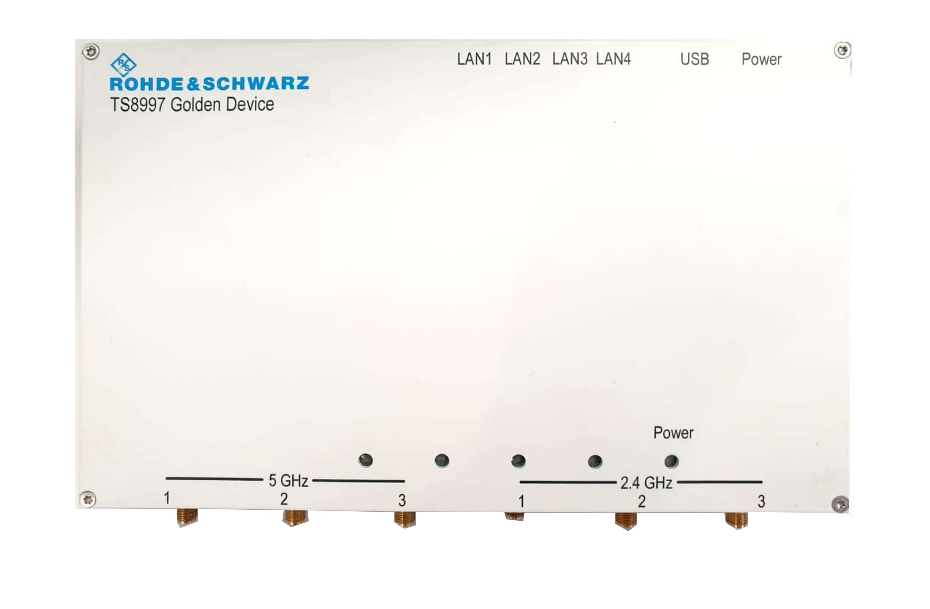
\includegraphics[width=0.55\textwidth]{fritz.pdf}
\caption{\acs{RS}\textregistered{} Golden device (\acs{CMW})}
\label{fig:cmwGUI}
\end{figure}

\section{Switching Units}
These Open Switch and Control Platform can be used to perform \acs{RF} switch and control tasks. This thesis uses two of these switching units. It is convenient to have a dedicated device instead of changing the setup for every test case like in the case of splitters and attenuators. The description and usage are explained below.

\subsection{\acs{RS}\textregistered{} \ac{OSP}-B157WN} \label{sec:wn}
This device switches between conducted measurements and normalized measurements. It allows us to select the appropriate/best antennas when performing normalized measurements and allows us to apply attenuation to the companion device (e.g. in case a real device instead of a \acs{CMW} test equipment is used). In the case of normalized measurements, it is programmed to automatically select the best probe antenna. The block diagram of the switching unit allows us to remotely control the device. The ANT ports are used for normalized measurements are connected to the antennas. The \acs{DUT} ports are used in case of conducted measurements. GEN W(8) is connected to the SMB 100A port of the \acs{OSP}-B157W8 which further connects the signal generator. The companion device can be connected to COMP 1 or COMP 2 but because reconnection is not possible during automation, the companion device is connected to the COMP 1 port of this switching module. The OUT ports are connected to \acs{OSP}-157W8 PORT ports.

\begin{figure}[H]
\centering
\includegraphics[width=0.74\textwidth]{ospwn.pdf}
\caption{Circuit diagram of the \acs{OSP}-B157WN board}
\label{fig:ospwn}
\end{figure}

I used the K-Tool at first to send \acs{SCPI} commands to the instrument to remotely switch between paths. The \acs{GUI} of the K-Tool is shown in the figure below. This tool allows users to add, connect, and send commands to the device remotely. The command to switch the path is as follows: 

\begin{lstlisting}[language=bash]
ROUTE: CLOSE(@F01M07(0602))
\end{lstlisting}

where, 602 stands for the name of the switch (i.e. K602) and 0 stands for the switch number (i.e. port 1 or 0). This command switches the path from OUT8 to DUT8. 

\begin{figure}[H]
\centering
\includegraphics[width=0.65\textwidth]{ktool.pdf}
\caption{K-Tool \acs{GUI}}
\label{fig:ktool}
\end{figure}

Further, I wrote a MATLAB\textregistered{} script to get the calibration values for each path switched. The calibration procedure uses the instrument to be calibrated (i.e. \acs{OSP}), signal generator, signal analyzer, and cables. Frequency response is generated for each path after measuring the power values for frequencies starting from 10 MHz up to 6 GHz with a step size of 10 MHz The cables are calibrated separately and subtracted from the final value to get the correct attenuation of the instrument. The frequency response is compared to the factory calibration values to check if the class which switches the instrument works fine. These calibration values are required at the later stage for normalization.

\subsection{\acs{RS}\textregistered{} \ac{OSP}-B157W8}
This device switches between the Signal Generator and Signal Analyzer depending on the test case (i.e. Receiver Blocking, Occupied Channel Bandwidth, Power, etc.). WMS32 software allows us to read out the calibration files from this switching module. It can also be done by using the correct \acs{SCPI} commands. The signal analyzer is connected to the Rx port of this device. The signal generator is connected to SMB 100A.

\begin{figure}[H]
\centering
\includegraphics[width=0.74\textwidth]{OSPW8.pdf}
\caption{Circuit diagram of \acs{OSP}-B157W8 diagram}
\label{fig:ospw8l}
\end{figure}



\section{\acs{RF} Shielded Box}
\acs{RS}\textregistered{} TS7124M features high shielding effectiveness over a wide frequency range (300 MHz to 6 GHz), the \acs{RF} test boxes allow measurements on different standards due to the supported frequency range. For radiation testing, the \acs{DUT} is inserted into the chamber using a drawer, which is closed by a tightly sealed door. Antennas installed on the inside of the \acs{RF} Shielded Box then interact with the \acs{DUT} by emitting or receiving electromagnetic radiation. The DUT is placed on a tray (Figure \ref{fig:yry}) within the RF shielded box.

\begin{figure}[H]
\centering
\includegraphics[width=0.55\textwidth]{tray.pdf}
\caption{ DUT holder tray (\acs{RS}\textregistered{} TS-F24P1)}
\label{fig:try}
\end{figure}

The antennas can be placed and oriented in a customer-specific geometrical arrangement. The box contains a full antenna ring where antennas can be mounted at 0$^{\circ}$, 45$^{\circ}$, and 90$^{\circ}$ tilt.  Submitting a \acs{DUT} to conducted instead of radiated RF signals via feedthroughs for \acs{RF} cables (or guiding conducted \acs{RF} signals away from the \acs{DUT}) can be applied as an alternative or supplement to antennas. The Figure \ref{fig:box} shows the antenna configuration used in this thesis.

\begin{figure}[H]
\centering
\includegraphics[width=0.55\textwidth]{chamber.pdf}
\caption{Full antenna ring with 6 vivaldi antennas}
\label{fig:box}
\end{figure}

In this thesis, broadband Vivaldi antennas are being used. The specification of the probe antennas (\acs{RS}\textregistered{} TS-F24-V2) are as follows: 


\begin{figure}[h]
    \begin{minipage}[c]{.7\textwidth}% or {.6\linewidth}, it's the same here
        \begin {tabular} {|l|l|} 
\toprule
Parameters & Value \\ 
\midrule 
Frequency & 2.4 to 16 GHz \\
VSWR (reflection coefficient) & $<$2; typ. 1.5 \\
Gain & 2 to 6 dBi (at 2.4 to 4 GHz)\\ 
 & 6 to 8 dBi (at 4 to 16 GHz)\\ 
Max. Input Power & 30 dBm (1 W) \\
Impedance & 50 $\Omega$ \\
Polarization & Linear (norm.)\\
\bottomrule
\end {tabular}    \end{minipage}
    \hfill
    \begin{minipage}[c]{.2\textwidth}
        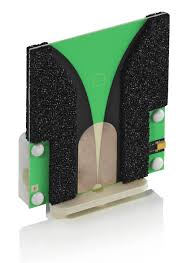
\includegraphics[width=\linewidth]{ProbeAntenna.jpg}
    \end{minipage}
    \caption{Specification of the Probe Antenna (\acs{RS}\textregistered{} - TS-F24-V2)}
\label{fig:probes}
\end{figure}      

\section{\ac{DUT}}
This thesis uses two DUTs (single antenna DUT and multi-antenna DUT) to investigate the measurement uncertainties introduced by conducted and normalized measurements. 

\begin{figure}[h]
    \begin{minipage}[c]{.7\textwidth}% or {.6\linewidth}, it's the same here
        \begin {tabular} {|l|l|} 
\toprule
Parameters & Value \\ 
\midrule 
Antenna type & detachable omni-directional \\
Antenna Gain & 3 dBi \\
Transmit Power & $<$ 20 dBm (\acs{EIRP})\\ 
Wireless Standards & \acs{IEEE} 802.11ac,a,n,g,b \\
Frequency & 2.4 and 5 GHz \\
\bottomrule
\end {tabular}    \end{minipage}
    \hfill
    \begin{minipage}[c]{.2\textwidth}
        \includegraphics[width=\linewidth]{SingleAntennaDUT.pdf}
    \end{minipage}
    \caption{Specification of the single-antenna \acs{DUT} (AC600 High Gain Wireless Dual Band USB Adapter, Archer T2UH)}
\label{fig:singleAntennaDUT}
\end{figure}     

\begin{figure}[h]
    \begin{minipage}[c]{.7\textwidth}% or {.6\linewidth}, it's the same here
        \begin {tabular} {|l|l|} 
\toprule
Parameters & Value \\ 
\midrule 
Antenna type & Omni-directional \\
Beamforming & Yes \\
Transmit Power &  $<$20 dBm (\acs{EIRP})\\ 
Wireless Standards & \acs{IEEE} 802.11ac,a,n,g,b \\
Frequency & 2.4 and 5 GHz \\
\bottomrule
\end {tabular}    \end{minipage}
    \hfill
    \begin{minipage}[c]{.2\textwidth}
        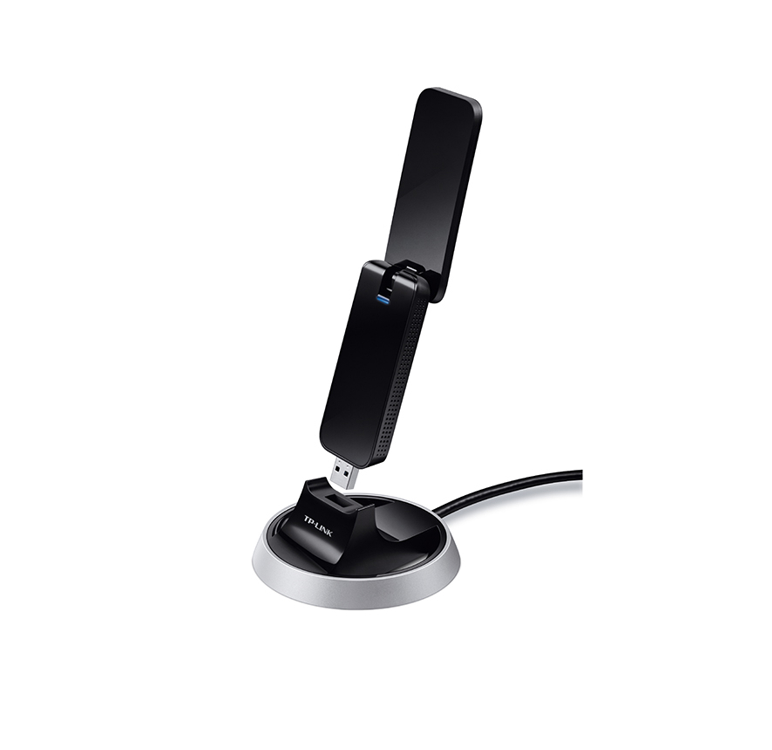
\includegraphics[width=\linewidth]{MultiAntennaDUT.pdf}
    \end{minipage}
    \caption{Specification of the multi-antenna \acs{DUT} (AC1900 High Gain Wireless Dual Band USB Adapter, Archer T9UH)}
\label{fig:multiAntennaDUT}
\end{figure}     
